\documentclass[]{ifjclass}
\usepackage{url}
\graphicspath{{pictures/}}
\usepackage{amsmath}
\usepackage{longtable}
\usepackage[clockwise]{rotating}
\usepackage{booktabs}
\usepackage{graphicx}   
\usepackage{pdflscape}
\newcommand{\h}[1]{\rotatebox{90}{\tm{#1}}}
\usepackage{array}
\newcommand{\h}[1]{\rotatebox{90}{\tm{#1}}} 
\newcommand{\nt}[1]{\ensuremath{\langle\text{#1}\rangle}}
\newcommand{\tm}[1]{\texttt{#1}}
\newcommand{\eps}{\ensuremath{\varepsilon}}
\newcounter{pravidlo}
\renewcommand{\thepravidlo}{\arabic{pravidlo}}
\newcommand{\rul}[2]{\refstepcounter{pravidlo}\thepravidlo.\quad & \nt{#1} &\rightarrow #2 \\}
\title{
    \logo\\[0.8cm]
    Dokumentace projektu z předmětů IFJ a IAL\\[1cm]
    \Large Varianta -- \texttt{TRP-izp}\\[0.25cm]
    \large Rozšíření: \texttt{BOOLTHEN}, \texttt{CONTROL}, \texttt{FUNEXP}
}

\vspace{1cm}
\author{\textbf{Ondřej Kvapil - xkvapio00 (281766)} 25\,\% \\ Filip Haza - xhazafi00 (281772) 25\,\% \\ Petr Nášel - xnaselp00 (270065) 25\,\% \\ Jonáš Ľalík - xlalikj00 (282341) 25\,\%}
\date{\vspace{0.75cm}\today}

\begin{document}
	\maketitle
    \newpage   
    \section{Obsah}
	\tableofcontents
    \newpage

    \section{Rozdělení práce}
        \begin{itemize}
        \item Filip Haza -- Lexikální analýza, tokenizace, main.c a Makefile. Vizualizace diagramu konečného automatu do dokumentace
        \item Petr Nášel -- Syntaktická analýza, precedenční analýza výrazů, abstraktní syntaktický strom. Vizualizace LL gramatiky, LL tabulky a precedenční tabulky do dokumentace.
        \item Jonáš Ľalík -- Sémantická analýza, tabulka symbolů nad hashovací tabulkou a chybové kódy. Vizualizace architektury překladače do dokumentace.
        \item Ondřej Kvapil -- Generátor cílového kódu, výpis instrukcí v IFJcode26, vestavěné funkce, main.c a Makefile
        \item Všichni -- Testy vlastních částí a celého překladače, PR review a dokumentace
        \end{itemize}

    \section{Spolupráce}
        \begin{itemize}
        \item \textbf{Komunikace} -- Jako hlavní komunikační kanál jsme používali Messenger skupinu. Pro online meetingy jsme používali Discord, ale také jsme komunikovali prostřednictvím komentářů v GitHub PR reviews, kde jsme přímo komentovali naši práci.
        \item \textbf{Code review a schvalování PR} -- Do main šel kód pouze přes Pull Requesty, ty potřebovali alespoň jedno schválení. Většinou od člena, kterého část se změnou pracovala. PR jsme procházeli na společných meetingách, pokud obsahovaly více nesrovnalostí, jinak pomocí komentářů přímo v Gitu
        \item \textbf{Testování} -- Celý překladač jsme ověřovali end2end testy pomocí skriptu, který výsledný kód spustil na Merlinovi v interpretu ic26int. Jednotlivé části jsme testovali unit testy.
        \item \textbf{Formátování} -- Zvolili jsme styl LLVM, pomocí nástroje clang-format.
        \end{itemize}
    \newpage
    \section{Architektura překladače}
    \begin{figure}[htbp]
        \centering
        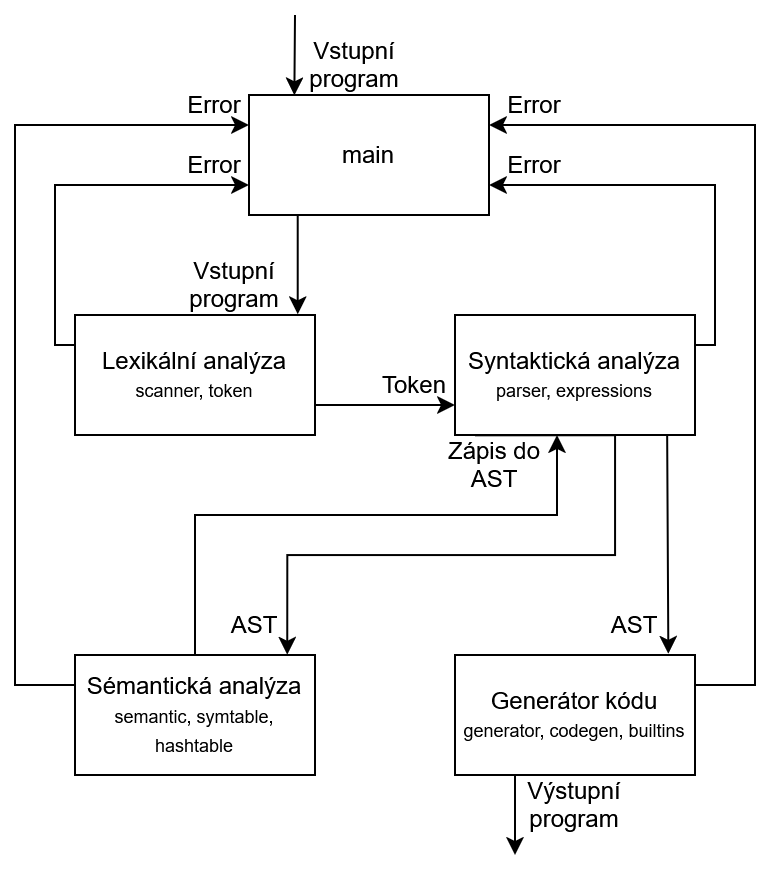
\includegraphics[width=\textwidth]{pictures/blokova_schema.png}
        \caption{Blokové schéma architektury překladače}
        \label{fig:architektura}
    \end{figure}
    \texttt{main} inicializuje scanner se zdrojovým programem. Scanner prochází zdrojovým programem a parser sestavuje AST pomocí tokenů ze scanneru. Při nalezení chyby v lexikální nebo syntaktické analýze je program ukončen s příslušnou chybou. Nad sestaveným AST proběhne sémantická analýza, která do něj zapisuje potřebné informace. Při nalezení chyby v sémantické analýze je do \texttt{main} vrácený typ chyby a program je ukončen. Nakonec generátor kódu, dle hotového AST, vygeneruje výsledný kód. Selhání generátoru kódu vrací \texttt{false} do \texttt{main} a program je ukončen.

    \newpage
    \section{Lexikální analýza}
        
        Lexikální analyzátor zpracovává vstupní proud znaků ze standardního vstupu, odstraňuje bílé znaky a komentáře, sleduje úroveň odsazení a na vyžádání předává syntaktickému analyzátoru lexikální jednotky ve formě struktury \texttt{Token} (nesoucí typ tokenu, číslo řádku a případnou sémantickou hodnotu).\par\medskip
        Lexikální analyzátor je navržen a implementován jako deterministický konečný automat (DKA) zobrazený na obrázku~\ref{fig:dka}. Některé lexikální konstrukce jazyka však nejsou v DKA realizovatelné (např. odsazování či vnořené komentáře), případně by jejich přímé vyjádření v~grafu vedlo ke zbytečnému nárůstu stavů. Reálná implementace se proto v~několika aspektech od standardního modelu DKA odlišuje -- tyto rozdíly jsou shrnuty v~sekci~\ref{subsec:odchylky}.\par\medskip
        \subsection{Diagram konečného automatu}
        \begingroup
        \makeatletter
        \setlength{\@fptop}{0pt}
        \setlength{\@fpbot}{0pt plus 1fil} % zarovná obrázek nahoru, dole nechá volné místo nad číslem stránky
        \makeatother
        \setlength{\abovecaptionskip}{8pt}
        \setlength{\belowcaptionskip}{0pt}
        \begin{figure}[p]
            \centering
            \vspace*{-1.8cm}
            \makebox[\textwidth][c]{%
                \rotatebox{-90}{%
                    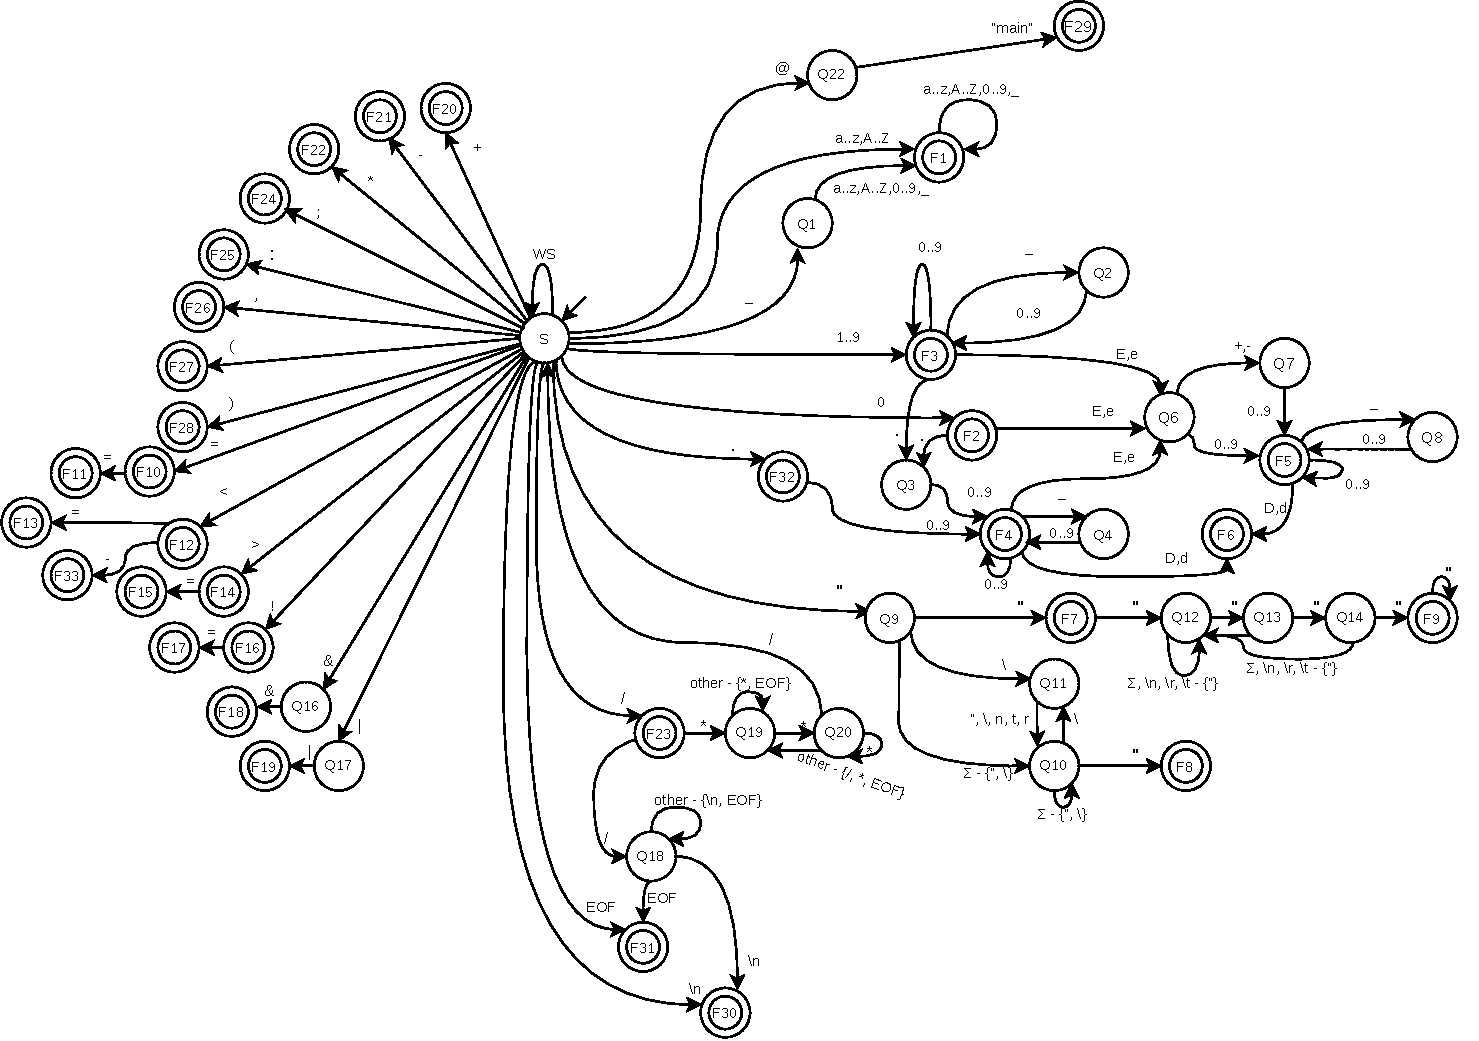
\includegraphics[page=1,width=.76\paperheight,height=.76\paperwidth,keepaspectratio]{Diagram_DKA.pdf}%
                }%
            }%
            \vspace{4pt}
            \caption{Diagram konečného automatu (DKA)}
            \label{fig:dka}
        \end{figure}
        \endgroup
        \clearpage

        \noindent\textbf{Legenda DKA:}\par\medskip
        \noindent Automat pracuje na principu hladového DKA (načítá nejdelší možný lexém). Z~důvodu přehlednosti grafu nejsou v~diagramu zakresleny přechody do chybového stavu:
        \begin{itemize}\setlength{\itemsep}{2pt}\setlength{\parskip}{0pt}
            \item \textbf{Neuvedené přechody v~mezistavech (\texttt{Q1}--\texttt{Q22}):} Přijde-li v~neakceptujícím stavu vstupní znak (nebo \texttt{EOF}), pro který z~daného stavu nevede žádná hrana, analyzátor hlásí lexikální chybu (\texttt{ERR\_LEXICAL}).
            \item \textbf{Ukončení v~koncových stavech (\texttt{F1}--\texttt{F33}):} Má-li akceptující stav odchozí hranu pro aktuální znak, automat pokračuje v~načítání. Jakmile přijde znak bez platného přechodu, vrátí se zpět na vstup pomocí funkce \texttt{ungetc()} (pokud se nemá zahodit) a výsledný token je předán syntaktickému analyzátoru.
        \end{itemize}
        \medskip
        \noindent
        \begin{minipage}[t]{0.49\textwidth}
        \footnotesize
        \begin{itemize}\setlength{\itemsep}{1pt}\setlength{\parskip}{0pt}
            \item \texttt{S} = \texttt{STATE\_START}
            \item \texttt{Q1} = \texttt{STATE\_UNDERSCORE}
            \item \texttt{Q2} = \texttt{STATE\_INT\_UNDERSCORE}
            \item \texttt{Q3} = \texttt{STATE\_NUM\_DOT}
            \item \texttt{Q4} = \texttt{STATE\_DOUBLE\_UNDERSCORE}
            \item \texttt{Q6} = \texttt{STATE\_EXPONENT}
            \item \texttt{Q7} = \texttt{STATE\_SIGN}
            \item \texttt{Q8} = \texttt{STATE\_EXP\_UNDERSCORE}
            \item \texttt{Q9} = \texttt{STATE\_QUOTE\_1}
            \item \texttt{Q10} = \texttt{STATE\_STRING}
            \item \texttt{Q11} = \texttt{STATE\_STRING\_ESCAPE}
            \item \texttt{Q12} = \texttt{STATE\_MSTR}
            \item \texttt{Q13} = \texttt{STATE\_MSTR\_END\_1}
            \item \texttt{Q14} = \texttt{STATE\_MSTR\_END\_2}
            \item \texttt{Q16} = \texttt{STATE\_AND} (\texttt{\&})
            \item \texttt{Q17} = \texttt{STATE\_OR} (\texttt{|})
            \item \texttt{Q18} = \texttt{STATE\_COM\_LINE}
            \item \texttt{Q19} = \texttt{STATE\_COM\_BLOCK}
            \item \texttt{Q20} = \texttt{STATE\_COM\_BLOCK\_STAR}
            \item \texttt{Q22} = \texttt{STATE\_ANNOT}
            \item \texttt{F1} = \texttt{STATE\_KW\_IDENTIFIER}
            \item \texttt{F2} = \texttt{STATE\_ZERO}
            \item \texttt{F3} = \texttt{STATE\_INT}
            \item \texttt{F4} = \texttt{STATE\_DOUBLE}
            \item \texttt{F5} = \texttt{STATE\_EXPONENT\_FINAL}
            \item \texttt{F6} = \texttt{STATE\_D\_SUFIX}
            \item \texttt{F7} = \texttt{STATE\_QUOTE\_2}
        \end{itemize}
        \end{minipage}%
        \hfill
        \begin{minipage}[t]{0.49\textwidth}
        \footnotesize
        \begin{itemize}\setlength{\itemsep}{1pt}\setlength{\parskip}{0pt}
            \item \texttt{F8} = \texttt{STATE\_STRING\_FINAL}
            \item \texttt{F9} = \texttt{STATE\_MSTR\_EXTRA\_QUOTE}
            \item \texttt{F10} = \texttt{STATE\_ASSIGN} (\texttt{=})
            \item \texttt{F11} = operátor \texttt{==}
            \item \texttt{F12} = \texttt{STATE\_LESS\_THAN} (\texttt{<})
            \item \texttt{F13} = operátor \texttt{<=}
            \item \texttt{F14} = \texttt{STATE\_GREATER\_THAN} (\texttt{>})
            \item \texttt{F15} = operátor \texttt{>=}
            \item \texttt{F16} = \texttt{STATE\_NOT} (\texttt{!})
            \item \texttt{F17} = operátor \texttt{!=}
            \item \texttt{F18} = operátor \texttt{\&\&}
            \item \texttt{F19} = operátor \texttt{||}
            \item \texttt{F20} = \texttt{STATE\_PLUS} (\texttt{+})
            \item \texttt{F21} = \texttt{STATE\_MINUS} (\texttt{-})
            \item \texttt{F22} = \texttt{STATE\_MULTIPLY} (\texttt{*})
            \item \texttt{F23} = \texttt{STATE\_SLASH} (\texttt{/})
            \item \texttt{F24} = \texttt{STATE\_SEMICOLON} (\texttt{;})
            \item \texttt{F25} = \texttt{STATE\_COLON} (\texttt{:})
            \item \texttt{F26} = \texttt{STATE\_COMMA} (\texttt{,})
            \item \texttt{F27} = \texttt{STATE\_LPAR} (\texttt{(})
            \item \texttt{F28} = \texttt{STATE\_RPAR} (\texttt{)})
            \item \texttt{F29} = \texttt{STATE\_ANNOT\_MAIN}
            \item \texttt{F30} = \texttt{STATE\_EOL} (\texttt{\textbackslash n})
            \item \texttt{F31} = \texttt{STATE\_EOF} (\texttt{EOF})
            \item \texttt{F32} = \texttt{STATE\_DOT\_CHECK} (\texttt{.})
            \item \texttt{F33} = operátor \texttt{<-}
        \end{itemize}
        \end{minipage}
        \normalsize
        \newpage

        \subsection{Odchylky od standardního DKA}\label{subsec:odchylky}
        \begin{itemize}
    \item \textbf{Zpracování víceřádkových řetězců:} V~implementaci se navíc po dosažení koncového stavu každá další bezprostředně navazující uvozovka \texttt{"} rovnou zapisuje do dynamického bufferu jako součást výsledného textu.

    \item \textbf{Řešení odsazování pomocí zásobníku:} Odsazování bloků není možné zachytit v~DKA, proto je řešeno přímo ve stavu \texttt{STATE\_START} pomocí zásobníku odsazení. Na začátku řádku scanner sečte úvodní mezery (tabulátory na začátku řádku nejsou povoleny a vedou k~\texttt{ERR\_LEXICAL}) a výsledek porovná s~vrcholem zásobníku, podle čehož vygeneruje \texttt{TOKEN\_INDENT} nebo \texttt{TOKEN\_DEDENT}. Prázdné řádky a řádky obsahující jen komentář odsazení nijak neovlivňují a do zásobníku se neukládají.

    \item \textbf{Dynamický buffer (\texttt{scanner\_buffer\_t}):} Slouží k~načítání lexémů s~proměnnou délkou (číselných literálů, řetězců a identifikátorů).

    \item \textbf{Rozlišení klíčových slov a identifikátorů:} V~implementaci i~diagramu DKA mají identifikátory a~klíčová slova společné stavy. Jejich rozlišení je řešeno před odesláním tokenu porovnáním načteného lexému s~tabulkou klíčových slov, na jehož základě se odešle buď token klíčového slova, nebo token identifikátoru s~atributem načteným z~dynamického bufferu.

    \item \textbf{Sloučení stavů pro zjednodušení kódu:} Některé stavy z~automatu byly v~implementaci sloučeny do jednoho, např. u~dvouznakových operátorů -- načte se první znak a~v~příslušném stavu se poté načte další znak a~vyhodnotí se, který token se má odeslat.

    \item \textbf{Vnořené blokové komentáře:} Zanořené blokové komentáře jsou v~implementaci řešeny pomocí celočíselného čítače \texttt{comment\_depth}. Blokový komentář neskončí, dokud není \texttt{comment\_depth = 0}.

    \item \textbf{Podmíněné generování \texttt{EOL} a~\texttt{EOF}:} Přechody do stavů pro \texttt{EOL} a~\texttt{EOF} neplatí bez výjimky. Token \texttt{EOL} se negeneruje na prázdných řádcích ani při více odřádkováních za sebou. Před vrácením samotného \texttt{EOF} zase analyzátor nejprve postupně vyprázdní zásobník odsazení a~odešle všechny zbývající tokeny \texttt{TOKEN\_DEDENT}.

    \item \textbf{Kontrola závorek (\texttt{bracket\_depth}):} Čítač vnoření kulatých závorek (\texttt{(...)}) ovlivňuje generování konců řádků i~kontrolu odsazení. Uvnitř závorek (\texttt{bracket\_depth > 0}) se negenerují tokeny \texttt{TOKEN\_EOL}, \texttt{TOKEN\_INDENT} ani \texttt{TOKEN\_DEDENT} a~nemění se zásobník odsazení. Analyzátor ale i~nadále zakazuje tabulátory a~hlídá, aby pokračovací řádky byly odsazené více než začátek logického řádku (uzavírací \texttt{)} přitom může být zarovnaná na jeho úroveň).
\end{itemize}

    \newpage
    \section{Syntaktická analýza}
        \subsection{LL Gramatika}
Syntaktická analýza struktury programu je realizována metodou rekurzivního sestupu na základě níže uvedené LL(1) gramatiky. 
Zpracování výrazů je z~LL(1) gramatiky vyčleněno a řešeno precedenční syntaktickou analýzou. Styčný symbol \textit{expr} označuje předání řízení funkci \texttt{parse\_expression}, zatímco symbol \textit{expr\_cont} představuje volání \texttt{parse\_expression\_from}, které navazuje na již načtený identifikátor či volání funkce a dokončí analýzu zbývající části výrazu.

Z~důvodu čitelnosti gramatiky jsou některé kontextové detaily řešeny přímo v~implementaci parseru:
\begin{itemize}\setlength{\itemsep}{2pt}\setlength{\parskip}{0pt}
    \item U~pravidla pro prolog (\textit{import}) parser dodatečně ověřuje, že identifikátor má přesnou hodnotu \texttt{ifj26} a že za symbolem \texttt{*} následuje \texttt{EOL} nebo \texttt{\$}.
    \item V~seznamech parametrů (\textit{params}) a argumentů (\textit{args}) je koncová čárka před \texttt{)} povolena pouze při odřádkování, což parser ověřuje porovnáním čísel řádků tokenů.
    \item Oddělení definic a příkazů na témže řádku středníkem \texttt{;} je vynucováno sledováním čísla řádku posledního zpracovaného tokenu.
\end{itemize}
\begin{longtable}{r l c l}
\caption{Pravidla LL(1) gramatiky jazyka IFJ26} \label{tab:ll-grammar} \\
\toprule
\textbf{Č.} & \textbf{Neterminál} & & \textbf{Pravá strana pravidla} \\
\midrule
\endfirsthead

\toprule
\textbf{Č.} & \textbf{Neterminál} & & \textbf{Pravá strana pravidla} \\
\midrule
\endhead

\midrule

\endfoot

\bottomrule
\endlastfoot

1.  & \textit{program}       & $\rightarrow$ & \textit{import} \textit{def\_list} \texttt{\$} \\
2.  & \textit{import}        & $\rightarrow$ & \texttt{import} \texttt{id} \texttt{.} \texttt{*} \\
3.  & \textit{def\_list}     & $\rightarrow$ & \texttt{EOL} \textit{def\_list} \\
4.  & \textit{def\_list}     & $\rightarrow$ & \textit{func\_main} \textit{sep\_opt} \textit{def\_list} \\
5.  & \textit{def\_list}     & $\rightarrow$ & \textit{func\_def} \textit{sep\_opt} \textit{def\_list} \\
6.  & \textit{def\_list}     & $\rightarrow$ & $\varepsilon$ \\
7.  & \textit{func\_main}    & $\rightarrow$ & \texttt{@main} \textit{eol\_list} \textit{func\_def} \\
8.  & \textit{func\_def}     & $\rightarrow$ & \texttt{def} \texttt{id} \texttt{(} \textit{params} \texttt{)} \textit{ret\_type\_opt} \texttt{=} \textit{func\_body} \\
9.  & \textit{params}        & $\rightarrow$ & \texttt{id} \texttt{:} \textit{type} \textit{params\_next} \\
10. & \textit{params}        & $\rightarrow$ & $\varepsilon$ \\
11. & \textit{params\_next}  & $\rightarrow$ & \texttt{,} \textit{params} \\
12. & \textit{params\_next}  & $\rightarrow$ & $\varepsilon$ \\
13. & \textit{ret\_type\_opt}& $\rightarrow$ & \texttt{:} \textit{type} \\
14. & \textit{ret\_type\_opt}& $\rightarrow$ & $\varepsilon$ \\
15. & \textit{func\_body}    & $\rightarrow$ & \textit{block} \\
16. & \textit{func\_body}    & $\rightarrow$ & \textit{value\_or\_if} \\
17. & \textit{type}          & $\rightarrow$ & \texttt{Int} \\
18. & \textit{type}          & $\rightarrow$ & \texttt{String} \\
19. & \textit{type}          & $\rightarrow$ & \texttt{Double} \\
20. & \textit{type}          & $\rightarrow$ & \texttt{Unit} \\
21. & \textit{type}          & $\rightarrow$ & \texttt{Boolean} \\
22. & \textit{block}         & $\rightarrow$ & \texttt{EOL} \texttt{INDENT} \textit{stmt\_list} \textit{dedent\_opt} \\
23. & \textit{dedent\_opt}   & $\rightarrow$ & \texttt{DEDENT} \\
24. & \textit{dedent\_opt}   & $\rightarrow$ & $\varepsilon$ \\
25. & \textit{stmt\_list}    & $\rightarrow$ & \texttt{EOL} \textit{stmt\_list} \\
26. & \textit{stmt\_list}    & $\rightarrow$ & \textit{statement} \textit{sep\_opt} \textit{stmt\_list} \\
27. & \textit{stmt\_list}    & $\rightarrow$ & $\varepsilon$ \\
28. & \textit{body}          & $\rightarrow$ & \textit{block} \\
29. & \textit{body}          & $\rightarrow$ & \textit{statement} \\
30. & \textit{statement}     & $\rightarrow$ & \texttt{val} \texttt{id} \textit{ret\_type\_opt} \texttt{=} \textit{value\_or\_if} \\
31. & \textit{statement}     & $\rightarrow$ & \texttt{var} \texttt{id} \textit{ret\_type\_opt} \texttt{=} \textit{value\_or\_if} \\
32. & \textit{statement}     & $\rightarrow$ & \textit{if\_state} \\
33. & \textit{statement}     & $\rightarrow$ & \textit{while\_state} \\
34. & \textit{statement}     & $\rightarrow$ & \textit{for\_state} \\
35. & \textit{statement}     & $\rightarrow$ & \textit{return\_state} \\
36. & \textit{statement}     & $\rightarrow$ & \texttt{id} \textit{id\_tail} \\
37. & \textit{statement}     & $\rightarrow$ & \textit{expr} \\
38. & \textit{id\_tail}      & $\rightarrow$ & \texttt{=} \textit{value\_or\_if} \\
39. & \textit{id\_tail}      & $\rightarrow$ & \textit{func\_call} \textit{expr\_cont} \\
40. & \textit{id\_tail}      & $\rightarrow$ & \textit{expr\_cont} \\
41. & \textit{if\_state}     & $\rightarrow$ & \texttt{if} \textit{expr} \texttt{then} \textit{body} \textit{eol\_list} \textit{else\_opt} \\
42. & \textit{else\_opt}     & $\rightarrow$ & \texttt{else} \textit{body} \\
43. & \textit{else\_opt}     & $\rightarrow$ & $\varepsilon$ \\
44. & \textit{while\_state}  & $\rightarrow$ & \texttt{while} \textit{expr} \texttt{do} \textit{body} \\
45. & \textit{for\_state}    & $\rightarrow$ & \texttt{for} \textit{for\_head} \\
46. & \textit{for\_head}     & $\rightarrow$ & \texttt{EOL} \textit{eol\_list} \texttt{INDENT} \textit{for\_gen} \textit{eol\_list} \\
    &                        &               & \textit{for\_guards\_ml} \texttt{DEDENT} \textit{eol\_list} \texttt{do} \textit{body} \\
47. & \textit{for\_head}     & $\rightarrow$ & \textit{for\_gen} \textit{for\_guards} \texttt{do} \textit{body} \\
48. & \textit{for\_gen}      & $\rightarrow$ & \texttt{id} \texttt{<-} \textit{expr} \textit{for\_dir} \textit{expr} \textit{for\_step\_opt} \\
49. & \textit{for\_dir}      & $\rightarrow$ & \texttt{to} \\
50. & \textit{for\_dir}      & $\rightarrow$ & \texttt{until} \\
51. & \textit{for\_step\_opt}& $\rightarrow$ & \texttt{by} \textit{expr} \\
52. & \textit{for\_step\_opt}& $\rightarrow$ & $\varepsilon$ \\
53. & \textit{for\_guards}   & $\rightarrow$ & \texttt{if} \textit{expr} \textit{for\_guards} \\
54. & \textit{for\_guards}   & $\rightarrow$ & $\varepsilon$ \\
55. & \textit{for\_guards\_ml}& $\rightarrow$ & \texttt{if} \textit{expr} \textit{eol\_list} \textit{for\_guards\_ml} \\
56. & \textit{for\_guards\_ml}& $\rightarrow$ & $\varepsilon$ \\
57. & \textit{return\_state} & $\rightarrow$ & \texttt{return} \textit{ret\_val} \\
58. & \textit{ret\_val}      & $\rightarrow$ & \textit{value\_or\_if} \\
59. & \textit{ret\_val}      & $\rightarrow$ & $\varepsilon$ \\
60. & \textit{value\_or\_if}  & $\rightarrow$ & \textit{if\_state} \\
61. & \textit{value\_or\_if}  & $\rightarrow$ & \textit{expr} \\
62. & \textit{func\_call}    & $\rightarrow$ & \texttt{(} \textit{args} \texttt{)} \\
63. & \textit{args}          & $\rightarrow$ & \textit{expr} \textit{args\_next} \\
64. & \textit{args}          & $\rightarrow$ & $\varepsilon$ \\
65. & \textit{args\_next}    & $\rightarrow$ & \texttt{,} \textit{args} \\
66. & \textit{args\_next}    & $\rightarrow$ & $\varepsilon$ \\
67. & \textit{sep\_opt}      & $\rightarrow$ & \texttt{;} \\
68. & \textit{sep\_opt}      & $\rightarrow$ & $\varepsilon$ \\
69. & \textit{eol\_list}     & $\rightarrow$ & \texttt{EOL} \textit{eol\_list} \\
70. & \textit{eol\_list}     & $\rightarrow$ & $\varepsilon$ \\
\end{longtable}

        \newpage
\clearpage
\subsection{LL Tabulka}

\begin{table}[!ht]
\centering
\caption{Prediktivní LL tabulka}
\label{tab:ll-tabulka}
\small
\setlength{\tabcolsep}{3pt}
\renewcommand{\arraystretch}{1.1}
\resizebox{\textwidth}{!}{%
\begin{tabular}{l|*{32}{c}}
\toprule
 & \h{import} & \h{@main} & \h{def} & \h{val} & \h{var} & \h{if} & \h{else} & \h{while} & \h{for} & \h{do} & \h{to} & \h{until} & \h{by} & \h{return} & \h{Int} & \h{String} & \h{Double} & \h{Unit} & \h{Boolean} & \h{id} & \h{lit} & \h{op} & \h{(} & \h{)} & \h{,} & \h{:} & \h{=} & \h{;} & \h{EOL} & \h{INDENT} & \h{DEDENT} & \h{\$} \\
\midrule
\nt{program} &  1 & & & & & & & & & & & & & & & & & & & & & & & & & & & & & & &  \\
\nt{import} &  2 & & & & & & & & & & & & & & & & & & & & & & & & & & & & & & &  \\
\nt{def\_list} &  & 4 & 5 & & & & & & & & & & & & & & & & & & & & & & & & & & 3 & & & 6  \\
\nt{func\_main} &  & 7 & & & & & & & & & & & & & & & & & & & & & & & & & & & & & &  \\
\nt{func\_def} &  & & 8 & & & & & & & & & & & & & & & & & & & & & & & & & & & & &  \\
\nt{params} &  & & & & & & & & & & & & & & & & & & & 9 & & & & 10 & & & & & & & &  \\
\nt{params\_next} &  & & & & & & & & & & & & & & & & & & & & & & & 12 & 11 & & & & & & &  \\
\nt{ret\_type\_opt} &  & & & & & & & & & & & & & & & & & & & & & & & & & 13 & 14 & & & & &  \\
\nt{func\_body} &  & & & & & 16 & & & & & & & & & & & & & & 16 & 16 & & 16 & & & & & & 15 & & &  \\
\nt{type} &  & & & & & & & & & & & & & & 17 & 18 & 19 & 20 & 21 & & & & & & & & & & & & &  \\
\nt{block} &  & & & & & & & & & & & & & & & & & & & & & & & & & & & & 22 & & &  \\
\nt{dedent\_opt} &  & & & & & & & & & & & & & & & & & & & & & & & & & & & & & & 23 & 24  \\
\nt{stmt\_list} &  & & & 26 & 26 & 26 & & 26 & 26 & & & & & 26 & & & & & & 26 & 26 & & 26 & & & & & & 25 & & 27 & 27  \\
\nt{body} &  & & & 29 & 29 & 29 & & 29 & 29 & & & & & 29 & & & & & & 29 & 29 & & 29 & & & & & & 28 & & &  \\
\nt{statement} &  & & & 30 & 31 & 32 & & 33 & 34 & & & & & 35 & & & & & & 36 & 37 & & 37 & & & & & & & & &  \\
\nt{id\_tail} &  & & & & & & 40 & & & & & & & & & & & & & & & 40 & 39 & & & & 38 & 40 & 40 & & 40 & 40  \\
\nt{if\_state} &  & & & & & 41 & & & & & & & & & & & & & & & & & & & & & & & & & &  \\
\nt{else\_opt} &  & 43 & 43 & 43 & 43 & 43 & 42 & 43 & 43 & & & & & 43 & & & & & & 43 & 43 & & 43 & & & & & 43 & 43 & & 43 & 43  \\
\nt{while\_state} &  & & & & & & & 44 & & & & & & & & & & & & & & & & & & & & & & & &  \\
\nt{for\_state} &  & & & & & & & & 45 & & & & & & & & & & & & & & & & & & & & & & &  \\
\nt{for\_head} &  & & & & & & & & & & & & & & & & & & & 47 & & & & & & & & & 46 & & &  \\
\nt{for\_gen} &  & & & & & & & & & & & & & & & & & & & 48 & & & & & & & & & & & &  \\
\nt{for\_dir} &  & & & & & & & & & & 49 & 50 & & & & & & & & & & & & & & & & & & & &  \\
\nt{for\_step\_opt} &  & & & & & 52 & & & & 52 & & & 51 & & & & & & & & & & & & & & & & 52 & & 52 &  \\
\nt{for\_guards} &  & & & & & 53 & & & & 54 & & & & & & & & & & & & & & & & & & & & & &  \\
\nt{for\_guards\_ml} &  & & & & & 55 & & & & & & & & & & & & & & & & & & & & & & & & & 56 &  \\
\nt{return\_state} &  & & & & & & & & & & & & & 57 & & & & & & & & & & & & & & & & & &  \\
\nt{ret\_val} &  & & & & & 58 & 59 & & & & & & & & & & & & & 58 & 58 & & 58 & & & & & 59 & 59 & & 59 & 59  \\
\nt{value\_or\_if} &  & & & & & 60 & & & & & & & & & & & & & & 61 & 61 & & 61 & & & & & & & & &  \\
\nt{func\_call} &  & & & & & & & & & & & & & & & & & & & & & & 62 & & & & & & & & &  \\
\nt{args} &  & & & & & & & & & & & & & & & & & & & 63 & 63 & & 63 & 64 & & & & & & & &  \\
\nt{args\_next} &  & & & & & & & & & & & & & & & & & & & & & & & 66 & 65 & & & & & & &  \\
\nt{sep\_opt} &  & 68 & 68 & 68 & 68 & 68 & & 68 & 68 & & & & & 68 & & & & & & 68 & 68 & & 68 & & & & & 67 & 68 & & 68 & 68  \\
\nt{eol\_list} &  & 70 & 70 & 70 & 70 & 70 & 70 & 70 & 70 & 70 & & & & 70 & & & & & & 70 & 70 & & 70 & & & & & 70 & 69 & 70 & 70 & 70  \\
\bottomrule
\end{tabular}%
}
\end{table}
        \newpage
        \subsection{Precedenční tabulka} 
        \begin{table}[htbp]
        \newpage
    \centering
    \small
    \setlength{\tabcolsep}{4pt}
    \begin{tabular}{|c||c|c|c|c|c|c|c|c|c|c|c|c|c|c|}
        \hline
        & \textbf{+} & \textbf{-} & \textbf{*} & \textbf{/} & \textbf{AND} & \textbf{OR} & \textbf{NOT}
        & \textbf{r} & \textbf{e} & \textbf{uminus} & \textbf{(} & \textbf{)} & \textbf{i} & \textbf{\$} \\
        \hline\hline
        \textbf{+}     & R & R & S & S & R & R & S & R & R & S & S & R & S & R \\ \hline
        \textbf{-}     & R & R & S & S & R & R & S & R & R & S & S & R & S & R \\ \hline
        \textbf{*}     & R & R & R & R & R & R & S & R & R & S & S & R & S & R \\ \hline
        \textbf{/}     & R & R & R & R & R & R & S & R & R & S & S & R & S & R \\ \hline
        \textbf{AND}   & S & S & S & S & R & R & S & S & S & S & E & R & S & R \\ \hline
        \textbf{OR}    & S & S & S & S & S & R & R & S & S & S & E & R & S & R \\ \hline
        \textbf{NOT}   & R & R & R & R & R & R & S & R & R & S & E & R & S & R \\ \hline
        \textbf{r}     & S & S & S & S & R & R & S & X & R & S & S & R & S & R \\ \hline
        \textbf{e}     & S & S & S & S & R & R & S & S & X & S & S & R & S & R \\ \hline
        \textbf{uminus}& R & R & R & R & R & R & S & R & R & S & S & R & S & R \\ \hline
        \textbf{(}     & S & S & S & S & R & R & R & S & S & S & S & E & S & X \\ \hline
        \textbf{)}     & R & R & R & R & S & S & S & R & R & X & X & R & X & R \\ \hline
        \textbf{i}     & R & R & R & R & R & R & R & R & R & X & X & R & X & R \\ \hline
        \textbf{\$}    & S & S & S & S & S & S & S & S & S & S & S & X & S & X \\ \hline
    \end{tabular}
    \caption{Precedenční tabulka}
    \label{tab:precedence}
    \end{table}

    \noindent
    Legenda: \textbf{R} -- redukce ($>$), \textbf{S} -- shift ($<$),
    \textbf{E} -- rovnost ($=$), \textbf{X} -- chyba.
    
    
    \newpage
    \section{Popis jednotlivých modulů}
        \begin{itemize}
        \item \textbf{ast.c/h} -- Modul ast definuje datové struktury abstraktního syntaktického stromu (AST) pro jednotlivé konstrukce jazyka IFJ26 (funkce, bloky, příkazy, výrazy) spolu s funkcemi pro jejich alokaci a rekurzivní uvolňování paměti.
        \item \textbf{builtins.c/h} -- Modul \texttt{builtins} implementuje generování kódu vestavěných funkcí jazyka IFJ26. Jednoduché funkce překládá přímo na posloupnost instrukcí v IFJcode26 a funkce \texttt{subStr} a \texttt{ord} generuje jednou na konci programu jako podprogramy, které se volají instrukcí \texttt{CALL}. Argumenty těchto dvou funkcí jsou předávány přes zásobník.
        \item \textbf{codegen.c/h} -- Modul \texttt{codegen} obsahuje pro každou instrukci IFJcode26 samostatnou funkci, která ji vypíše na standartní výstup. Ostatní části překladače díky němu nemusí řešit formát instrukcí. Přiděluje unikátní čísla návěštím a převádí konstanty do požadovaného tvaru.
        \item \textbf{errors.h} -- Hlavičkový soubor definující výčtový typ se všemi návratovými kódy překladače v souladu se specifikací.
        \item \textbf{expressions.c/h} -- Modul expressions implementuje precedenční syntaktickou analýzu (PSA) aritmetických, relačních a logických výrazů pomocí zásobníku a precedenční tabulky. Zpracovává také vnořená volání funkcí a unární operátory a výsledný výraz vrací jako podstrom AST.
        \item \textbf{generator.c/h} -- Modul \texttt{generator} prochází AST a pro každý jeho uzel vygeneruje odpovídající instrukce v IFJcode26, přičemž výrazy počítá na zásobníku. Každé funkci připraví vlastní rámec se všemi proměnnými a odlišuje jejich unikátní id ze sémantické analýzy. Dále se stará o automatický převod Int na Double, vyhodnocování operátorů AND, OR a kontrolu nulového kroku ve for cyklu.
        \item \textbf{hashtable.c/h} -- Modul \texttt{hashtable} implementuje ADT vyhledávací tabulky, která přiřazuje klíč typu string ukazateli na data neznámého typu, používá otevřené adresování, kolize řeší dvojitou rozptylovací funkcí, roste po prvočíselních velikostech od \texttt{101} do \texttt{55889} před dosažením poloviční kapacity.
        
        \item \textbf{main.c} -- Vstupní bod překladače, inicializuje lexikální analyzátor nad standartním vstupem. Spouští syntaktickou analýzu, která vytváří AST, jeho sémantickou analýzu a generování cílového kódu. Následně vrací odpovídající návratový kód.
        \item \textbf{parser.c/h} -- Parser metodou rekurzivního sestupu (top-down) kontroluje syntaxi tokenů ze skeneru. Sestavuje abstraktní syntaktický strom (AST), který je poté předáván jiným modulům k dalšímu zpracování.
        \item \textbf{scanner.c/h} -- Modul \texttt{scanner} implementuje lexikální analýzu vstupního programu napsaného v jazyce IFJ26 pomocí DKA a prostřednictvím funkce \texttt{get\_next\_token()} vrací syntaktickému analyzátoru načtený lexém v podobě tokenu.
        \item \textbf{semantic.c/h} -- Modul \texttt{semantic} implementuje sémantickou analýzu programu napsaného v jazyce IFJ26 rekurzivním průchodem AST, přičemž kontroluje sémantické chyby a zapisuje typ každého výrazu, unikátní id proměnných a odvozené návratové typy funkcí do AST.
        
        \item \textbf{symtable.c/h} -- Modul \texttt{symtable} implementuje ADT tabulky symbolů postavené nad \texttt{hashtable}, udržuje zásobník rozsahů platnosti, každý rozsah má vyhledávací tabulku, která drží jeho symboly, a rozsahy jsou prohledávány od nejvnitřnějšího směrem ven.
        
        \item \textbf{token.c/h} -- Modul \texttt{token} definuje rozhraní mezi lexikálním a syntaktickým analyzátorem. Hlavičkový soubor \texttt{token.h} obsahuje výčet typů tokenů a strukturu \texttt{Token}, která uchovává typ lexému, číslo řádku a případně i atribut. Soubor \texttt{token.c} zajišťuje uvolnění dynamicky alokované paměti tokenů.
        \item \textbf{types.h} -- Hlavičkový soubor, který definuje datové typy jazyka IFJ26. Doplněný o pomocné typy Unknown a Any, které sdílí sémantická analýza a generátor kódu.
        \end{itemize}
    \newpage
    \section{Využití AI}
        \subsection{Použité modely}
            Claude - Opus 5.5, Sonnet 5.5, Fable 5.2 \\
            Gemini - 3.1.Pro, Hydrogen 4
        \subsection{Způsob využití}
            \textbf{Postup:} nastudování problému; konkrétní dotaz AI pro hlubší pochopení; pokud jsme nevěděli, jak na konkrétní implementaci, požádali jsme AI o logický postup nebo v některých případech blok kódu
            \par\medskip 
            \noindent AI nám byla nápomocná dovysvětlením zadání. Dále také k hledání chyb, jak v našem kódu, tak v kódu kolegů. Velkou roli hrála ve tvorbě testů
        \subsection{Problémy ve využití}
            Jediný problém, na který jsme narazili, byl v případě generování end-to-end testů.I přes to, že měl agent k dispozici zadání, generoval testy, které s ním nebyly v souladu a ukazoval falešné chyby.
        \subsection{Code review}
            Kvůli bezpečnějšímu přístupu jsme AI posílali hotové části kódu pro schválení.V případě chyb jsme je konzultovali mezi sebou.
    \newpage
    \section{Zdroje}
    [1] MohamedTaha98. \textit{djb2 hash function.c}. Online. Dostupné z: \url{https://gist.github.com/MohamedTaha98/ccdf734f13299efb73ff0b12f7ce429f}. [citováno 2026-10-06]

\end{document}



